\mode
<article>

%% Markup
\markdownSetupSnippet{horizontalRule/singleFrame}{snippet=witiko/beamer/MU/horizontalRule/singleFrame}

%% Title page
\maketitle

\mode
<presentation>

%% Markup
\markdownSetupSnippet{horizontalRule/frameBreak}{snippet=witiko/beamer/MU/horizontalRule/frameBreak}
\markdownSetupSnippet{headingTwo/several}{snippet=witiko/beamer/MU/headingTwo/several}

%% Title page
\begin{frame}[plain]
\begin{tikzpicture}[overlay, remember picture]
  \node[anchor=south east, xshift=204.5pt, yshift=-27pt] at (current page.south east) {
    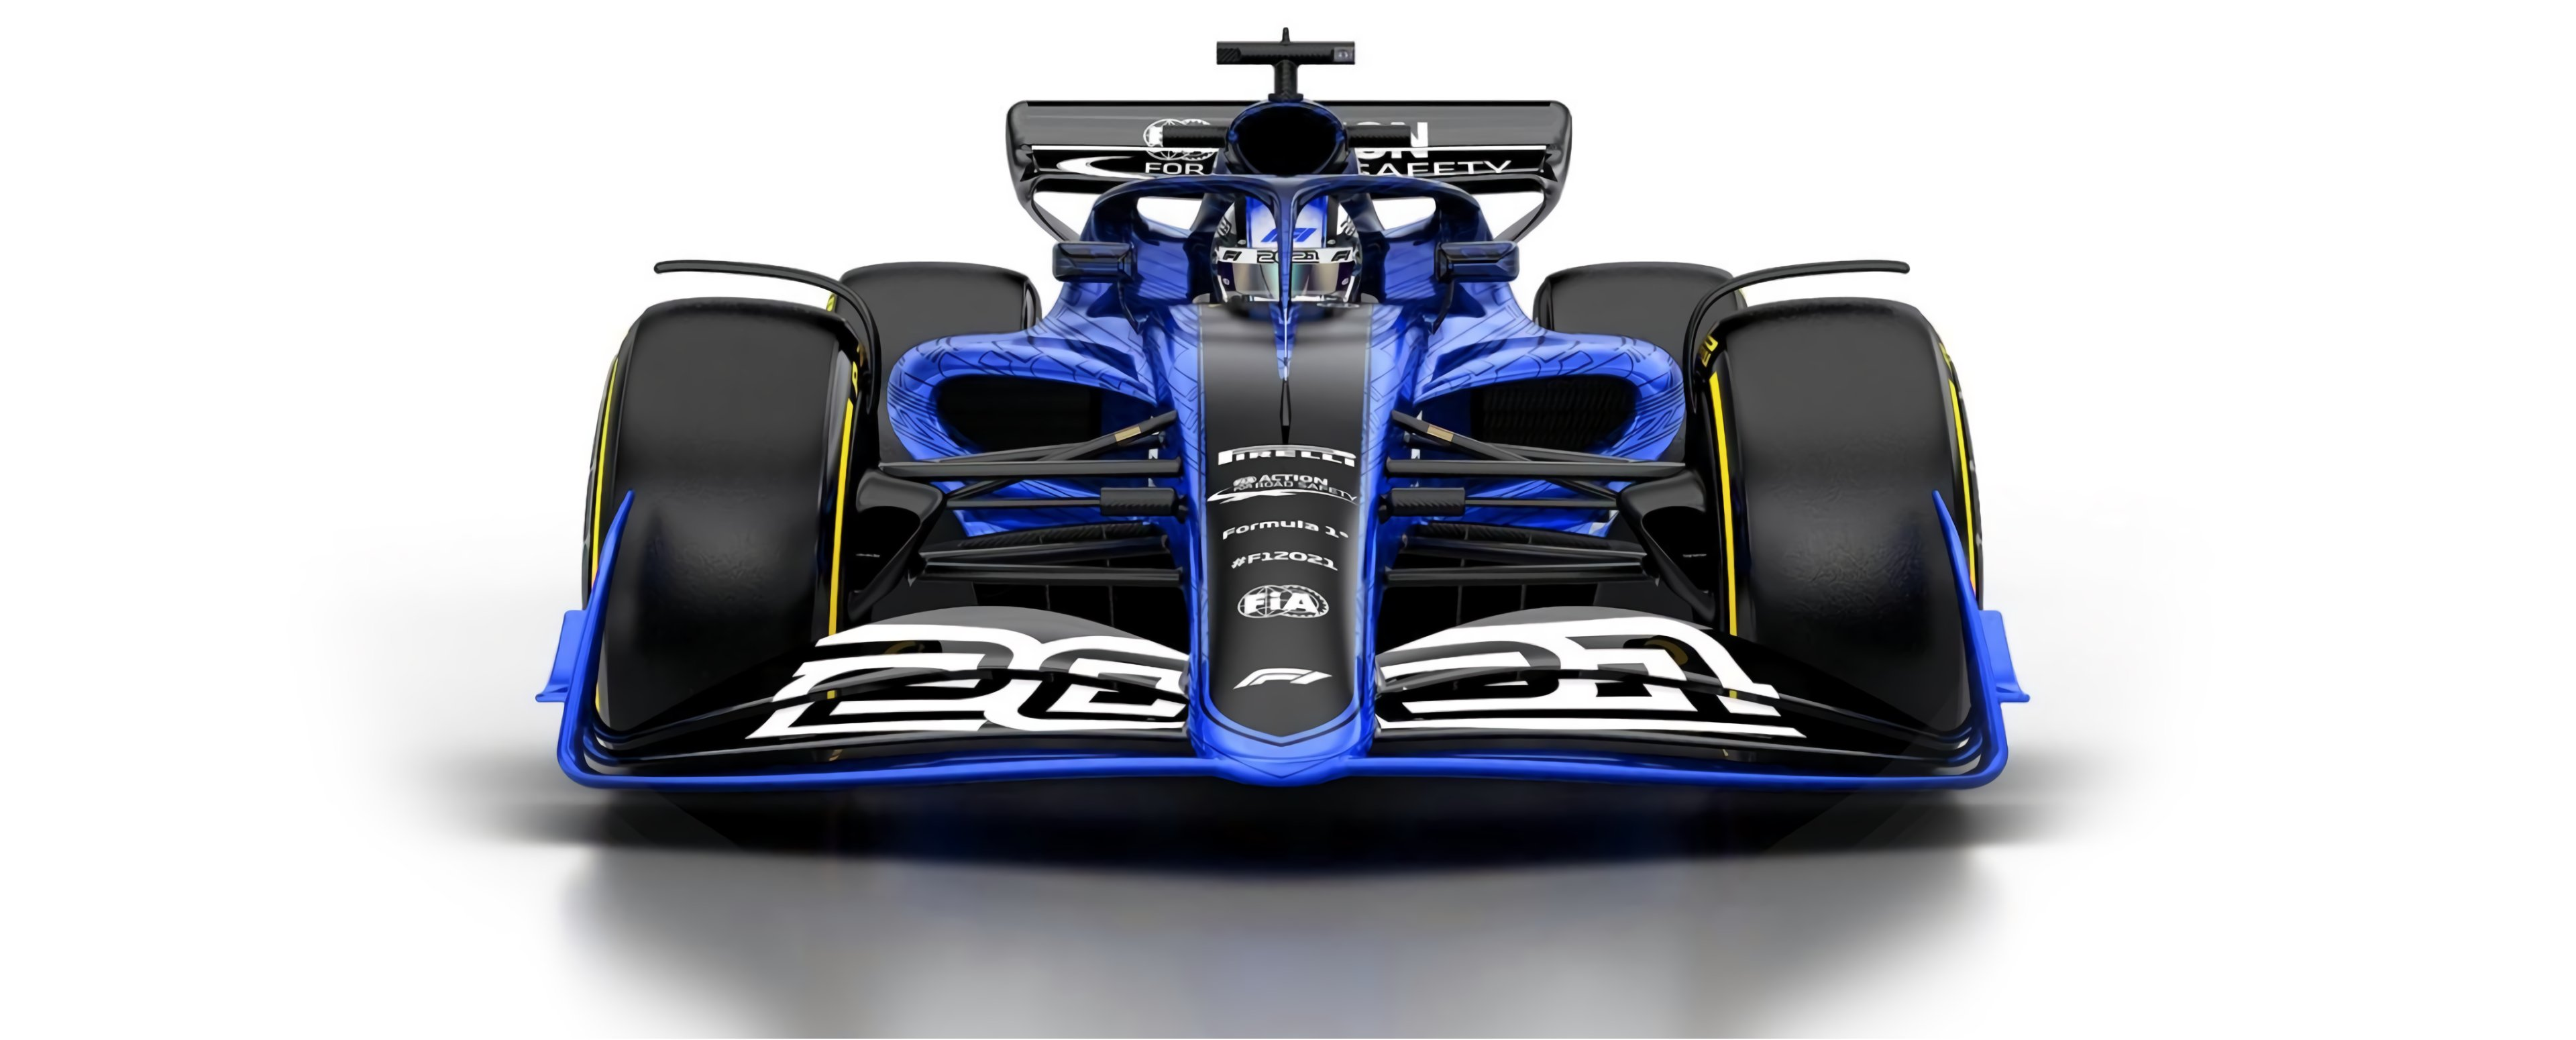
\includegraphics[height=0.91\textheight]{formula1}
  };
\end{tikzpicture}
\maketitle
\end{frame}

%% Graphics
\setkeys{Gin}{
  width = \columnwidth,
  height = \paperheight,
  keepaspectratio,
}

\mode
<article>

% Introduction
\markdownInput[slice=^ introduction]{presentation.md}

\printbibliography

\mode
<presentation>

\section{Introduction}
\begin{frame}[fragile]
  \markdownInput[slice=introduction]{presentation.md}
\end{frame}

\begin{frame}[plain]
\vfill\vfill
\centerline{Thank You for Your Attention!}
\vfill\vfill\vfill
\end{frame}

\part{\bibname}
\frame{\vfill\partpage\vfill}

\section{\bibname}
\begin{frame}[allowframebreaks]{\bibname}
\printbibliography[heading=none]
\end{frame}

\mode
<all>
